\chapter{\StructuresChapterName}

\RU{В принципе, структура в \CCpp это, с некоторыми допущениями, просто всегда лежащий рядом, 
и в той же последовательности, набор переменных, не обязательно одного типа
\footnote{\ac{AKA} \q{гетерогенный контейнер}}.}
\EN{A \CCpp structure, with some assumptions, is just a set of variables, always stored
in memory together, not necessary of the same type
\footnote{\ac{AKA} \q{heterogeneous container}}.}

% sections
\section{MSVC: \RU{Пример SYSTEMTIME}\EN{SYSTEMTIME example}}
\label{sec:SYSTEMTIME}

\newcommand{\FNSYSTEMTIME}{\footnote{\href{http://msdn.microsoft.com/en-us/library/ms724950(VS.85).aspx}{MSDN: SYSTEMTIME structure}}}

\RU{Возьмем, к примеру, структуру SYSTEMTIME\FNSYSTEMTIME{} из win32 описывающую время.}
\EN{Let's take SYSTEMTIME\FNSYSTEMTIME{} win32 structure describing time.}

\RU{Она объявлена так:}\EN{That's how it is defined:}

\begin{lstlisting}[caption=WinBase.h]
typedef struct _SYSTEMTIME {
  WORD wYear;
  WORD wMonth;
  WORD wDayOfWeek;
  WORD wDay;
  WORD wHour;
  WORD wMinute;
  WORD wSecond;
  WORD wMilliseconds;
} SYSTEMTIME, *PSYSTEMTIME;
\end{lstlisting}

\RU{Пишем на Си функцию для получения текущего системного времени:}
\EN{Let's write a C function to get current time:}

\lstinputlisting{patterns/15_structs/1_systemtime/systemtime.c}

\RU{Что в итоге}\EN{We got} (MSVC 2010):

\lstinputlisting[caption=MSVC 2010 /GS-]{patterns/15_structs/1_systemtime/systemtime.asm}

\RU{Под структуру в стеке выделено 16 байт ~--- именно столько будет \TT{sizeof(WORD)*8}
(в структуре 8 переменных с типом WORD).}
\EN{16 bytes are allocated for this structure in local stack~---that is exactly \TT{sizeof(WORD)*8}
(there are 8 WORD variables in the structure).}

\newcommand{\FNMSDNGST}{\footnote{\href{http://msdn.microsoft.com/en-us/library/ms724390(VS.85).aspx}{MSDN: GetSystemTime function}}}

\RU{Обратите внимание на тот факт, что структура начинается с поля \TT{wYear}. 
Можно сказать, что в качестве аргумента для \TT{GetSystemTime()}\FNMSDNGST передается указатель на структуру 
SYSTEMTIME, но можно также сказать, что передается указатель на поле \TT{wYear}, 
что одно и тоже! 
\TT{GetSystemTime()} пишет текущий год в тот WORD на который указывает переданный указатель, 
затем сдвигается на 2 байта вправо, пишет текущий месяц, и т.д., и т.д.}
\EN{Pay attention to the fact the structure beginning with \TT{wYear} field.
It can be said, an pointer to SYSTEMTIME structure is passed to the \TT{GetSystemTime()}\FNSYSTEMTIME,
but it is also can be said, pointer to the \TT{wYear} field is passed, and that is the same!
\TT{GetSystemTime()} writes current year to the WORD pointer pointing to, then shifts 2 bytes
ahead, then writes current month, etc, etc.}

\subsection{\olly}
\index{\olly}

\RU{Компилируем этот пример в}\EN{Let's compile this example in} MSVC 2010 \RU{с ключами}\EN{with} 
\TT{/GS- /MD} \RU{и запускаем в}\EN{keys and run it in} \olly.
\RU{Открываем окна данных и стека по адресу, который передается в качестве первого аргумента в ф-цию}
\EN{Let's open windows of data and stack at the address which is passed as the first argument into}
\TT{GetSystemTime()}\EN{ function}, 
\RU{ждем пока эта ф-ция исполнится, и видим следующее}\EN{let's wait until it's executed and we see this}:
\figname \ref{fig:struct_olly_1}.

\RU{Точное системнео время на моем компьютере, в которое исполнилась ф-ция, это}
\EN{Precise system time of function execution on my computer is} 5 \RU{июня}\EN{june} 2014, 7:17:45:
\figname \ref{fig:struct_olly_2}.

\RU{Таким образом, в окне данных мы видим следующие 16 байт}\EN{So we see these 16 bytes in the
data window}: 
\begin{lstlisting}
DE 07 06 00 04 00 04 00
07 00 11 00 2D 00 8D 00
\end{lstlisting}

\RU{Каждые два байта отражают одно поле структуры}\EN{Each two bytes representing one structure field}. 
\RU{А так как порядок байт (\gls{endianness}) \IT{little endian},
то в начале следует младший байт, затем старший}\EN{Since \gls{endianness} is \IT{little endian}, 
we see low byte first and then high one}.
\RU{Следовательно, вот какие 16-битные числа сейчас записаны в памяти}
\EN{Hence, these are values which are currently stored in memory}:

\begin{center}
\begin{tabular}{ | l | l | l | }
\hline
\headercolor{} \RU{Шестнадцатиричное число}\EN{Hexadecimal number} & 
\headercolor{} \RU{десятичное число}\EN{decimal number} & 
\headercolor{} \RU{имя поля}\EN{field name} \\
\hline
0x07DE & 2014	& wYear \\
\hline
0x0006 & 6	& wMonth \\
\hline
0x0004 & 4	& wDayOfWeek \\
\hline
0x0005 & 5	& wDay \\
\hline
0x0007 & 7	& wHour \\
\hline
0x0011 & 17	& wMinute \\
\hline
0x002D & 45	& wSecond \\
\hline
0x008D & 141	& wMilliseconds \\
\hline
\end{tabular}
\end{center}

\RU{В окне стека, видны те же значения, только они сгруппированы как 32-битные значения}
\EN{The same values are seen in the stack window, but they are groupped as 32-bit values}.

\RU{Затем}\EN{And then} \printf \RU{просто берет нужные значения и выводит их на консоль}
\EN{just takes values it needs and outputs them to the console}.

\RU{Некоторые поля}{Some values} \printf \RU{не выводит}{doesn't output} (\TT{wDayOfWeek} \AndENRU 
\TT{wMilliseconds}), \RU{но они находятся в памяти и доступны для использования}{but they are
in memory right now, available for using}.

\begin{figure}[H]
\centering
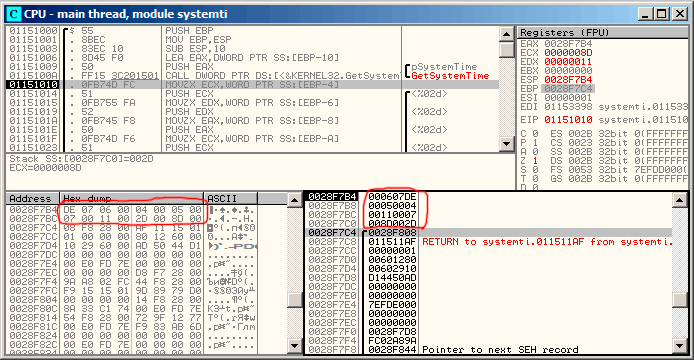
\includegraphics[scale=\FigScale]{patterns/15_structs/1_systemtime/olly_systemtime1.png}
\caption{\olly: \TT{GetSystemTime()} \RU{только что исполнилась}\EN{just executed}}
\label{fig:struct_olly_1}
\end{figure}

\begin{figure}[H]
\centering
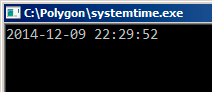
\includegraphics[scale=0.66]{patterns/15_structs/1_systemtime/olly_systemtime2.png}
\caption{\olly: \RU{Вывод \printf}\EN{\printf output}}
\label{fig:struct_olly_2}
\end{figure}

\subsection{\RU{Замена структуры массивом}\EN{Replacing the structure by array}}

\RU{Тот факт, что поля структуры это просто переменные расположенные рядом, 
я могу проиллюстрировать следующим образом.}
\EN{The fact the structure fields are just variables located side-by-side, 
I can demonstrate by the following technique.}
\RU{Глядя на описание структуры}\EN{Keeping in ming} \TT{SYSTEMTIME}
\RU{, я могу переписать этот простой пример так:}
\EN{ structure description, I can rewrite this simple example like this:}

\lstinputlisting{patterns/15_structs/1_systemtime/systemtime2.c}

\RU{Компилятор немного поворчит:}\EN{Compiler will grumble for a little:}

\begin{lstlisting}
systemtime2.c(7) : warning C4133: 'function' : incompatible types - from 'WORD [8]' to 'LPSYSTEMTIME'
\end{lstlisting}

\RU{Тем не менее, выдаст такой код}\EN{But nevertheless, it will produce this code}:

\lstinputlisting[caption=MSVC 2010]{patterns/15_structs/1_systemtime/systemtime2.asm}

\RU{И это работает так же}\EN{And it works just as the same}!

\RU{Любопытно что результат на ассемблере неотличим от предыдущего}
\EN{It is very interesting fact the
result in assembly form cannot be distinguished from the result of previous compilation}.
\RU{Таким образом, глядя на этот код, 
никогда нельзя сказать с уверенностью, была ли там объявлена структура, либо просто набор переменных.}
\EN{So by looking at this code, one cannot say for sure, was there structure declared, or just pack of variables.} 

\RU{Тем не менее, никто в здравом уме делать так не будет}
\EN{Nevertheless, no one will do it in sane state of mind}.
\RU{Потому что это неудобно}\EN{Since it is not convenient}. 
\RU{К тому же, иногда, поля в структуре могут меняться разработчиками, 
переставляться местами, и т.д}\EN{Also structure fields may be changed by developers, swapped, etc}.

\RU{Я не привожу здесь пример с \olly, потому что он будет точно такой же, как и в случае со структурой.}
\EN{I'm not adding \olly example here, because it will be just as the same as in the case 
with structure.}


\section{\RU{Выделяем место для структуры через malloc()}\EN{Let's allocate space for a structure using malloc()}}
\label{struct_malloc_example}

\RU{Однако, бывает и так, что проще хранить структуры не в стеке, а в \glslink{heap}{куче}:}
\EN{Sometimes it is simpler to place structures not the in local stack, but in the \gls{heap}:}

\lstinputlisting{patterns/15_structs/2_using_malloc/systemtime_malloc.c}

\RU{Скомпилируем на этот раз с оптимизацией (\Ox) чтобы было проще увидеть то, что нам нужно.}
\EN{Let's compile it now with optimization (\Ox) so it would be easy see what we need.}

\lstinputlisting[caption=\Optimizing MSVC]{patterns/15_structs/2_using_malloc/systemtime_malloc.asm}

\index{\CStandardLibrary!malloc()}
\RU{Итак, \TT{sizeof(SYSTEMTIME) = 16}, именно столько байт выделяется при помощи \TT{malloc()}. 
Она возвращает указатель на только что выделенный блок памяти в \EAX, который копируется в \ESI. 
Win32 функция \TT{GetSystemTime()} обязуется сохранить состояние \ESI, 
поэтому здесь оно нигде не сохраняется и продолжает использоваться после вызова \TT{GetSystemTime()}.}
\EN{So, \TT{sizeof(SYSTEMTIME) = 16} and that is exact number of bytes to be allocated by \TT{malloc()}.
It returns a pointer to a freshly allocated memory block in the \EAX register,
which is then moved into the \ESI register.
\TT{GetSystemTime()} win32 function takes care of saving value in \ESI,
and that is why it is not saved here and continues to be used after the \TT{GetSystemTime()} call.}

\index{x86!\Instructions!MOVZX}
\RU{
Новая инструкция ~--- \MOVZX (\IT{Move with Zero eXtend}). 
Она нужна почти там же где и \MOVSX, 
только всегда очищает остальные биты в 0. Дело в том, что \printf требует 32-битный тип \Tint, 
а в структуре лежит WORD ~--- это 16-битный беззнаковый тип. Поэтому копируя значение из WORD в \Tint, 
нужно очистить биты от 16 до 31, иначе там будет просто случайный мусор, оставшийся от предыдущих действий 
с регистрами.}
\EN{New instruction~---\MOVZX (\IT{Move with Zero eXtend}).
It may be used in most cases as \MOVSX, but it sets the remaining bits to 0.
That's because \printf requires a 32-bit \Tint, but we got a WORD in the structure~---that
is 16-bit unsigned type.
That's why by copying the value from a WORD into \Tint{}, bits from 16 to 31 must be cleared, 
because a random noise may be there, which is left from the previous operations on the register(s).}

\RU{В этом примере можно также представить структуру как массив 8-и WORD-ов:}
\EN{In this example, it's possible to represent the structure as an array of 8 WORDs:}

\lstinputlisting{patterns/15_structs/2_using_malloc/systemtime_malloc2.c}

\RU{Получим такое}\EN{We get}:

\lstinputlisting[caption=\Optimizing MSVC]{patterns/15_structs/2_using_malloc/systemtime_malloc2.asm}

\RU{И снова мы получаем идентичный код, неотличимый от предыдущего.}
\EN{Again, we got the code cannot be distinguished from the previous one.}
\RU{Но и снова нужно отметить, что в реальности так лучше не делать, 
если только вы не знаете точно, что вы делаете.}
\EN{And again it should be noted, you haven't to do this in practice, unless you really know what you are doing.}


\subsection{UNIX: struct tm}

% subsections here:
\EN{\subsection{Linux}

Let's take the \TT{tm} structure from \TT{time.h} in Linux for example:

\lstinputlisting{patterns/15_structs/3_tm_linux/GCC_tm.c}

Let's compile it in GCC 4.4.1:

\lstinputlisting[caption=GCC 4.4.1]{patterns/15_structs/3_tm_linux/GCC_tm_EN.asm}

Somehow, \IDA did not write the local variables' names in the local stack.
But since we already are experienced reverse engineers :-) we may do it without this information in 
this simple example.

\myindex{x86!\Instructions!LEA}

Please also pay attention to the \TT{lea edx, [eax+76Ch]}~---this instruction just adds \TT{0x76C} (1900) to value in \EAX,
but doesn't modify any flags. See also the relevant section about \LEA{}~(\myref{sec:LEA}).

\subsubsection{GDB}

Let's try to load the example into GDB
\footnote{The \IT{date} result is slightly corrected for demonstration purposes.
Of course, it's not possible to run GDB that quickly, in the same second.}:

\lstinputlisting[caption=GDB]{patterns/15_structs/3_tm_linux/GCC_tm_GDB.txt}

We can easily find our structure in the stack.
First, let's see how it's defined in \IT{time.h}:

\begin{lstlisting}[caption=time.h, label=struct_tm]
struct tm
{
  int	tm_sec;
  int	tm_min;
  int	tm_hour;
  int	tm_mday;
  int	tm_mon;
  int	tm_year;
  int	tm_wday;
  int	tm_yday;
  int	tm_isdst;
};
\end{lstlisting}

Pay attention that
32-bit \Tint is used here instead of WORD in SYSTEMTIME.
So, each field occupies 32-bit.

Here are the fields of our structure in the stack:

\begin{lstlisting}
0xbffff0dc:	0x080484c3	0x080485c0	0x000007de	0x00000000
0xbffff0ec:	0x08048301	0x538c93ed	0x00000025 sec	0x0000000a min
0xbffff0fc:	0x00000012 hour	0x00000002 mday	0x00000005 mon 	0x00000072 year
0xbffff10c:	0x00000001 wday	0x00000098 yday	0x00000001 isdst0x00002a30
0xbffff11c:	0x0804b090	0x08048530	0x00000000	0x00000000
\end{lstlisting}

Or as a table:

\begin{center}
\begin{tabular}{ | l | l | l | }
\hline
\headercolor{} Hexadecimal number & 
\headercolor{} decimal number & 
\headercolor{} field name \\
\hline
0x00000025 & 37 	& tm\_sec \\
\hline
0x0000000a & 10 	& tm\_min \\
\hline
0x00000012 & 18 	& tm\_hour \\	
\hline
0x00000002 & 2 		& tm\_mday \\	
\hline
0x00000005 & 5 		& tm\_mon \\	
\hline
0x00000072 & 114 	& tm\_year \\
\hline
0x00000001 & 1 		& tm\_wday \\	
\hline
0x00000098 & 152 	& tm\_yday \\	
\hline
0x00000001 & 1 		& tm\_isdst \\
\hline
\end{tabular}
\end{center}

Just like SYSTEMTIME (\myref{sec:SYSTEMTIME}), 

there are also other fields available that are not used, like tm\_wday, tm\_yday, tm\_isdst.
}
\RU{\subsectionold{Linux}

В Линуксе, для примера, возьмем структуру \TT{tm} из \TT{time.h}:

\lstinputlisting{patterns/15_structs/3_tm_linux/GCC_tm.c}

Компилируем при помощи GCC 4.4.1:

\lstinputlisting[caption=GCC 4.4.1]{patterns/15_structs/3_tm_linux/GCC_tm_RU.asm}

К сожалению, по какой-то причине, \IDA не сформировала названия локальных переменных в стеке. 
Но так как мы уже опытные реверсеры :-) то можем обойтись и без этого в таком простом примере.

\myindex{x86!\Instructions!LEA}
Обратите внимание на \TT{lea edx, [eax+76Ch]} ~--- эта инструкция прибавляет \TT{0x76C} (1900) к \EAX, 
но не модифицирует флаги. См. также соответствующий раздел об инструкции \LEA{}~(\myref{sec:LEA}).


\subsubsectionold{GDB}

Попробуем загрузить пример в GDB
\footnote{Результат работы \IT{date} немного подправлен в целях демонстрации.
Конечно же, в реальности, нельзя так быстро запустить GDB, чтобы значение секунд осталось бы таким же.}:

\lstinputlisting[caption=GDB]{patterns/15_structs/3_tm_linux/GCC_tm_GDB.txt}

Мы легко находим нашу структуру в стеке.
Для начала, посмотрим, как она объявлена в \IT{time.h}:

\begin{lstlisting}[caption=time.h, label=struct_tm]
struct tm
{
  int	tm_sec;
  int	tm_min;
  int	tm_hour;
  int	tm_mday;
  int	tm_mon;
  int	tm_year;
  int	tm_wday;
  int	tm_yday;
  int	tm_isdst;
};
\end{lstlisting}

Обратите внимание что здесь 32-битные \Tint вместо WORD в SYSTEMTIME.
Так что, каждое поле занимает 32-битное слово.

Вот поля нашей структуры в стеке:

\begin{lstlisting}
0xbffff0dc:	0x080484c3	0x080485c0	0x000007de	0x00000000
0xbffff0ec:	0x08048301	0x538c93ed	0x00000025 sec	0x0000000a min
0xbffff0fc:	0x00000012 hour	0x00000002 mday	0x00000005 mon 	0x00000072 year
0xbffff10c:	0x00000001 wday	0x00000098 yday	0x00000001 isdst0x00002a30
0xbffff11c:	0x0804b090	0x08048530	0x00000000	0x00000000
\end{lstlisting}

Либо же, в виде таблицы:

\begin{center}
\begin{tabular}{ | l | l | l | }
\hline
\headercolor{} Шестнадцатеричное число & 
\headercolor{} десятичное число & 
\headercolor{} имя поля \\
\hline
0x00000025 & 37 	& tm\_sec \\
\hline
0x0000000a & 10 	& tm\_min \\
\hline
0x00000012 & 18 	& tm\_hour \\	
\hline
0x00000002 & 2 		& tm\_mday \\	
\hline
0x00000005 & 5 		& tm\_mon \\	
\hline
0x00000072 & 114 	& tm\_year \\
\hline
0x00000001 & 1 		& tm\_wday \\	
\hline
0x00000098 & 152 	& tm\_yday \\	
\hline
0x00000001 & 1 		& tm\_isdst \\
\hline
\end{tabular}
\end{center}

Как и в примере с SYSTEMTIME (\myref{sec:SYSTEMTIME}), здесь есть и другие поля, готовые для использования, 
но в нашем примере они не используются, например, tm\_wday, tm\_yday, tm\_isdst.
}
\EN{\subsubsection{ARM}

\myparagraph{\OptimizingKeilVI (\ThumbMode)}

Same example:

\lstinputlisting[caption=\OptimizingKeilVI (\ThumbMode)]{patterns/15_structs/3_tm_linux/ARM/tm_ARM_keil_thumb.asm}

\myparagraph{\OptimizingXcodeIV (\ThumbTwoMode)}

\IDA \q{knows} the \TT{tm} structure 
(because \IDA \q{knows} the types of the arguments of library functions like \TT{localtime\_r()}), 

so it shows here structure elements accesses and their names.

\lstinputlisting[caption=\OptimizingXcodeIV (\ThumbTwoMode)]{patterns/15_structs/3_tm_linux/ARM/tm_ARM_xcode_thumb.asm}
}
\RU{\subsection{ARM}

\subsubsection{\OptimizingKeilVI (\ThumbMode)}

Этот же пример:

\lstinputlisting[caption=\OptimizingKeilVI (\ThumbMode)]{patterns/15_structs/3_tm_linux/ARM/tm_ARM_keil_thumb.asm}

\subsubsection{\OptimizingXcodeIV (\ThumbTwoMode)}

\IDA \q{узнала} структуру \TT{tm} 
(потому что \IDA \q{знает} типы аргументов библиотечных функций, 
таких как \TT{localtime\_r()}), 
поэтому показала здесь обращения к отдельным элементам структуры и присвоила им имена
.

\lstinputlisting[caption=\OptimizingXcodeIV (\ThumbTwoMode)]{patterns/15_structs/3_tm_linux/ARM/tm_ARM_xcode_thumb.asm}
}
\EN{\subsectionold{MIPS}

\lstinputlisting[caption=\Optimizing GCC 4.4.5 (IDA),numbers=left]{patterns/15_structs/3_tm_linux/MIPS/MIPS_O3_IDA_EN.lst}

This is an example where the branch delay slots can confuse us.

For example, there is the instruction \q{addiu \$a1, 1900} at line 35 which adds 1900 to the year number.

It's executed before the corresponding JALR at line 34, do not forget about it.

}
\RU{\subsection{MIPS}

\lstinputlisting[caption=\Optimizing GCC 4.4.5 (IDA),numbers=left]{patterns/15_structs/3_tm_linux/MIPS/MIPS_O3_IDA_RU.lst}

Это тот пример, где branch delay slot-ы могут нас запутать.

Например, в строке 35 есть инструкция \q{addiu \$a1, 1900}, добавляющая 1900 к числу года.

Но она исполняется перед исполнением соответствующей JALR в строке 34, не забыайте.

}
% subsection:
\EN{\subsubsection{Structure as a set of values}

In order to illustrate that the structure is just variables laying side-by-side in one place, 
let's rework our example while looking at the \IT{tm} structure definition again: \lstref{struct_tm}.

\lstinputlisting{patterns/15_structs/3_tm_linux/as_array/GCC_tm2.c}

\myindex{\CStandardLibrary!localtime\_r()}
N.B. 
The pointer to the \TT{tm\_sec} field is passed into \TT{localtime\_r}, i.e., 
to the first element of the \q{structure}.

The compiler warns us:

\begin{lstlisting}[caption=GCC 4.7.3]
GCC_tm2.c: In function 'main':
GCC_tm2.c:11:5: warning: passing argument 2 of 'localtime_r' from incompatible pointer type [enabled by default]
In file included from GCC_tm2.c:2:0:
/usr/include/time.h:59:12: note: expected 'struct tm *' but argument is of type 'int *'
\end{lstlisting}

But nevertheless, it generates this:

\lstinputlisting[caption=GCC 4.7.3]{patterns/15_structs/3_tm_linux/as_array/GCC_tm2.asm}

This code is identical to what we saw previously and it is
not possible to say, was it a structure in original source code or just a pack of variables.

And this works. 
However, it is not recommended to do this in practice. 

Usually, non-optimizing compilers allocates variables in the local stack in the 
same order as they were declared in the function.

Nevertheless, there is no guarantee.

By the way, some other compiler may warn about the \TT{tm\_year}, \TT{tm\_mon}, \TT{tm\_mday},
\TT{tm\_hour}, \TT{tm\_min} variables, but not \TT{tm\_sec}
 are used without being initialized.

Indeed, the compiler is not aware that these are to be filled by\\
\TT{localtime\_r()} function.

We chose this example, since all structure fields are of type \Tint.%

This would not work if structure fields are 16-bit (\TT{WORD}), 
like in the case of the \TT{SYSTEMTIME} structure---\TT{GetSystemTime()} 
will fill them incorrectly 
(because the local variables are aligned on a 32-bit boundary).
Read more about it in next section: 
\q{\StructurePackingSectionName} (\myref{structure_packing}).

So, a structure is just a pack of variables laying on one place, side-by-side.
We could say that the structure is the instruction to the compiler, directing it to hold variables in one place.
By the way, in some very early C versions (before 1972), there were no structures at all \RitchieDevC.

There is no debugger example here: it is just the same as you already saw.

\subsubsection{Structure as an array of 32-bit words}

\lstinputlisting{patterns/15_structs/3_tm_linux/as_array/GCC_tm3.c}

We just \IT{cast} a pointer to structure to an array of \Tint{}'s.
And that works!
We run the example at 23:51:45 26-July-2014.

\begin{lstlisting}[label=GCC_tm3_output]
0x0000002D (45)
0x00000033 (51)
0x00000017 (23)
0x0000001A (26)
0x00000006 (6)
0x00000072 (114)
0x00000006 (6)
0x000000CE (206)
0x00000001 (1)
\end{lstlisting}

The variables here 
are in the same order as they are enumerated in the definition of the structure: \myref{struct_tm}.

Here is how it gets compiled:

\lstinputlisting[caption=\Optimizing GCC 4.8.1]{patterns/15_structs/3_tm_linux/as_array/GCC_tm3_EN.lst}

Indeed: the space in the local stack is first treated as a structure, and then it's treated as an array.

It's even possible to modify the fields of the structure through this pointer.

And again, it's dubiously hackish way to do things, not recommended for use in production code.

\mysubparagraph{\Exercise}

As an exercise, try to modify (increase by 1) the current month number, treating the structure as 
an array.

\subsubsection{Structure as an array of bytes}

We can go even further. Let's \IT{cast} the pointer to an array of bytes and dump it:

\lstinputlisting{patterns/15_structs/3_tm_linux/as_array/GCC_tm4.c}

\begin{lstlisting}
0x2D 0x00 0x00 0x00 
0x33 0x00 0x00 0x00 
0x17 0x00 0x00 0x00 
0x1A 0x00 0x00 0x00 
0x06 0x00 0x00 0x00 
0x72 0x00 0x00 0x00 
0x06 0x00 0x00 0x00 
0xCE 0x00 0x00 0x00 
0x01 0x00 0x00 0x00 
\end{lstlisting}

We also run this example also at 23:51:45 26-July-2014
\footnote{The time and date are the same for demonstration purposes. Byte values are fixed up.}.
The values are just the same as in the previous dump 
(\myref{GCC_tm3_output}), and of course, the lowest byte goes first, because this is a little-endian architecture 
(\myref{sec:endianness}).

\lstinputlisting[caption=\Optimizing GCC 4.8.1]{patterns/15_structs/3_tm_linux/as_array/GCC_tm4_EN.lst}
}
\RU{\subsection{Структура как набор переменных}

Чтобы проиллюстрировать то что структура ~--- это просто набор переменных, лежащих в одном месте, 
переделаем немного пример, еще раз заглянув в описание структуры \IT{tm}: \lstref{struct_tm}.

\lstinputlisting{patterns/15_structs/3_tm_linux/as_array/GCC_tm2.c}

\myindex{\CStandardLibrary!localtime\_r()}
N.B. В \TT{localtime\_r} передается указатель именно на \TT{tm\_sec}, 
т.е. на первый элемент \q{структуры}.

В итоге, и этот компилятор поворчит:

\begin{lstlisting}[caption=GCC 4.7.3]
GCC_tm2.c: In function 'main':
GCC_tm2.c:11:5: warning: passing argument 2 of 'localtime_r' from incompatible pointer type [enabled by default]
In file included from GCC_tm2.c:2:0:
/usr/include/time.h:59:12: note: expected 'struct tm *' but argument is of type 'int *'
\end{lstlisting}

Тем не менее, сгенерирует такое:

\lstinputlisting[caption=GCC 4.7.3]{patterns/15_structs/3_tm_linux/as_array/GCC_tm2.asm}

Этот код почти идентичен уже рассмотренному, и нельзя сказать, была ли структура
в оригинальном исходном коде либо набор переменных.

И это работает. 
Однако, в реальности так лучше не делать. 
Обычно, неоптимизируюий компилятор располагает переменные в локальном
стеке в том же порядке, в котором они объявляются в функции.

Тем не менее, никакой гарантии нет.

Кстати, какой-нибудь другой компилятор может предупредить, что переменные \TT{tm\_year}, \TT{tm\_mon}, \TT{tm\_mday},
\TT{tm\_hour}, \TT{tm\_min}, но не \TT{tm\_sec}, используются без инициализации.
Действительно, ведь компилятор не знает что они будут заполнены при вызове функции
\TT{localtime\_r()}.

Мы выбрали именно этот пример для иллюстрации, потому что все члены структуры имеют тип \Tint.
Это не сработает, если поля структуры будут иметь размер 16 бит (\TT{WORD}), как в случае
со структурой \TT{SYSTEMTIME}\EMDASH{}\TT{GetSystemTime()} 
заполнит их неверно 
(потому что локальные переменные выровнены по 32-битной границе).
Читайте об этом в следующей секции: 
\q{\StructurePackingSectionName} (\myref{structure_packing}).

Так что, структура --- это просто набор переменных лежащих в одном месте, рядом.

Можно было бы сказать, что структура --- это инструкция компилятору, заставляющая его удерживать переменные в одном месте.

Кстати, когда-то, в очень ранних версиях Си (перед 1972) структур не было вовсе \RitchieDevC.

Здесь нет примера с отладчиком: потому что он будет полностью идентичным тому, что вы уже видели.

\subsection{Структура как массив 32-битных слов}

\lstinputlisting{patterns/15_structs/3_tm_linux/as_array/GCC_tm3.c}

Мы просто приводим (\IT{cast}) указатель на структуру к массиву \Tint{}-ов.
И это работает!
Запускаем пример 23:51:45 26-July-2014.

\begin{lstlisting}[label=GCC_tm3_output]
0x0000002D (45)
0x00000033 (51)
0x00000017 (23)
0x0000001A (26)
0x00000006 (6)
0x00000072 (114)
0x00000006 (6)
0x000000CE (206)
0x00000001 (1)
\end{lstlisting}

Переменные здесь в том же порядке, в котором они перечислены в определении структуры: \myref{struct_tm}.

Вот как это компилируется:

\lstinputlisting[caption=\Optimizing GCC 4.8.1]{patterns/15_structs/3_tm_linux/as_array/GCC_tm3_RU.lst}

И действительно: место в локальном стеке в начале используется как структура, затем как массив.

Возможно даже модифицировать поля структуры через указатель.

И снова, это сомнительный хакерский способ, который не рекомендуется использовать в настоящем коде.

\myparagraph{\Exercise}

В качестве упражнения, попробуйте модифицировать (увеличить на 1) 
текущий номер месяца обращаясь со структурой как с массивом.

\subsection{Структура как массив байт}

Можно пойти еще дальше. Можно привести (\IT{cast}) указатель к массиву байт и вывести его:%

\lstinputlisting{patterns/15_structs/3_tm_linux/as_array/GCC_tm4.c}

\begin{lstlisting}
0x2D 0x00 0x00 0x00 
0x33 0x00 0x00 0x00 
0x17 0x00 0x00 0x00 
0x1A 0x00 0x00 0x00 
0x06 0x00 0x00 0x00 
0x72 0x00 0x00 0x00 
0x06 0x00 0x00 0x00 
0xCE 0x00 0x00 0x00 
0x01 0x00 0x00 0x00 
\end{lstlisting}

Мы также запускаем этот пример в 23:51:45 26-July-2014
\footnote{Время и дата такая же в целях демонстрации. Значения байт были подправлены.}.
Переменные точно такие же, как и в предыдущем выводе 
(\myref{GCC_tm3_output}), и конечно, младший байт идет в самом начале, потому что это архитектура 
little-endian (\myref{sec:endianness}).

\lstinputlisting[caption=\Optimizing GCC 4.8.1]{patterns/15_structs/3_tm_linux/as_array/GCC_tm4_RU.lst}
}


\section{\StructurePackingSectionName}

\RU{Достаточно немаловажный момент, это упаковка полей в структурах\footnote{См. также: \URLWPDA}.}
\EN{One important thing is fields packing in structures\footnote{See also: \URLWPDA}.}

\RU{Возьмем простой пример:}\EN{Let's take a simple example:}

\lstinputlisting{patterns/15_structs/4_packing/packing.c}

\RU{Как видно, мы имеем два поля \Tchar (занимающий один байт) и еще два ~--- \Tint (по 4 байта).}
\EN{As we see, we have two \Tchar fields (each is exactly one byte) and two more~---\Tint (each - 4 bytes).}

\subsection{x86}

\RU{Компилируется это все в:}\EN{That's all compiling into:}

\lstinputlisting{patterns/15_structs/4_packing/packing.asm}

\RU{Мы видим здесь что адрес каждого поля в структуре выравнивается по 4-байтной границе. 
Так что каждый \Tchar здесь занимает те же 4 байта что и \Tint. Зачем? 
Затем что процессору удобнее обращаться по таким адресам и кэшировать данные из памяти.}
\EN{As we can see, each field's address is aligned on a 4-bytes border.
That's why each \Tchar occupies 4 bytes here (like \Tint). Why?
Thus it is easier for CPU to access memory at aligned addresses and to cache data from it.}

\RU{Но это не экономично по размеру данных.}\EN{However, it is not very economical in size sense.}

\RU{Попробуем скомпилировать тот же исходник с опцией}\EN{Let's try to compile it with option} (\TT{/Zp1}) 
(\IT{/Zp[n] pack structures on n-byte boundary}).

\lstinputlisting[caption=MSVC /Zp1]{patterns/15_structs/4_packing/packing_msvc_Zp1.asm}

\RU{Теперь структура занимает 10 байт и все \Tchar занимают по байту. Что это дает? 
Экономию места. Недостаток ~--- процессор будет обращаться к этим полям не так эффективно 
по скорости, как мог бы.}
\EN{Now the structure takes only 10 bytes and each \Tchar value takes 1 byte. What it give to us?
Size economy. And as drawback~---CPU will access these fields without maximal performance it can.}

\RU{Как нетрудно догадаться, если структура используется много в каких исходниках и объектных файлах, 
все они должны быть откомпилированы с одним и тем же соглашением об упаковке структур.}
\EN{As it can be easily guessed, if the structure is used in many source and object files,
all these must be compiled with the same convention about structures packing.}

\newcommand{\FNURLMSDNZP}{\footnote{\href{http://msdn.microsoft.com/en-us/library/ms253935.aspx}
{MSDN: Working with Packing Structures}}}
\newcommand{\FNURLGCCPC}{\footnote{\href{http://gcc.gnu.org/onlinedocs/gcc/Structure_002dPacking-Pragmas.html}
{Structure-Packing Pragmas}}}

\RU{Помимо ключа MSVC \TT{/Zp}, указывающего, по какой границе упаковывать поля структур, есть также 
опция компилятора \TT{\#pragma pack}, её можно указывать прямо в исходнике. 
Это справедливо и для MSVC\FNURLMSDNZP и GCC\FNURLGCCPC{}.}
\EN{Aside from MSVC \TT{/Zp} option which set how to align each structure field, here is also
\TT{\#pragma pack} compiler option, it can be defined right in source code.
It is available in both MSVC\FNURLMSDNZP and GCC\FNURLGCCPC{}.}

\RU{Давайте теперь вернемся к \TT{SYSTEMTIME}, которая состоит из 16-битных полей. 
Откуда наш компилятор знает что их надо паковать по однобайтной границе?}
\EN{Let's back to the \TT{SYSTEMTIME} structure consisting in 16-bit fields.
How our compiler know to pack them on 1-byte alignment boundary?}

\RU{В файле \TT{WinNT.h} попадается такое:}\EN{\TT{WinNT.h} file has this:}

\begin{lstlisting}[caption=WinNT.h]
#include "pshpack1.h"
\end{lstlisting}

\RU{И такое:}\EN{And this:}

\begin{lstlisting}[caption=WinNT.h]
#include "pshpack4.h"                   // 4 byte packing is the default
\end{lstlisting}

\RU{Сам файл PshPack1.h выглядит так:}\EN{The file PshPack1.h looks like:}

\begin{lstlisting}[caption=PshPack1.h]
#if ! (defined(lint) || defined(RC_INVOKED))
#if ( _MSC_VER >= 800 && !defined(_M_I86)) || defined(_PUSHPOP_SUPPORTED)
#pragma warning(disable:4103)
#if !(defined( MIDL_PASS )) || defined( __midl )
#pragma pack(push,1)
#else
#pragma pack(1)
#endif
#else
#pragma pack(1)
#endif
#endif /* ! (defined(lint) || defined(RC_INVOKED)) */
\end{lstlisting}

\RU{Собственно, так и задается компилятору, как паковать объявленные после \TT{\#pragma pack} структуры.}
\EN{That's how compiler will pack structures defined after \TT{\#pragma pack}.}

\subsection{ARM + \OptimizingKeil + \ThumbMode}

\lstinputlisting[caption=\OptimizingKeil + \ThumbMode]{patterns/15_structs/4_packing/packing_Keil_thumb.asm}

\RU{Как мы помним, здесь передается не указатель на структуру, а сама структура, а так как в ARM первые 4 аргумента
функции передаются через регистры, то поля структуры передаются через}
\EN{As we may recall, here a structure passed instead of pointer to structure,
and since first 4 function arguments in ARM are passed via registers,
so then structure fields are passed via} \TT{R0-R3}.

\index{ARM!\Instructions!LDRB}
\index{x86!\Instructions!MOVSX}
\RU{Инструкция }\TT{LDRB} \RU{загружает один байт из памяти и расширяет до 32-бит учитывая знак.}
\EN{loads one byte from memory and extending it to 32-bit, taking into account its sign.}
\RU{Это то же что и инструкция}\EN{This is akin to} \MOVSX \RU{в}\EN{instruction in} x86.
\RU{Она здесь применяется для загрузки полей}\EN{Here it is used for loading fields} $a$ \AndENRU $c$ 
\RU{из структуры}\EN{from structure}.

\index{Function epilogue}
\RU{Еще что бросается в глаза, так это то что вместо эпилога функции, переход на эпилог другой функции!}
\EN{One more thing we spot easily, instead of function epilogue, here is jump to another function's epilogue!}
\RU{Действительно, то была совсем другая, не относящаяся к этой, функция, однако, она имела точно такой же
эпилог}\EN{Indeed, that was quite different function, not related in any way to our function, however, it has exactly
the same epilogue} 
(\RU{видимо, тоже хранила в стеке 5 локальных переменных}\EN{probably because, it hold 5 local variables too} 
($5*4=0x14$)).
\RU{К тому же, она находится рядом (обратите внимание на адреса).}
\EN{Also it is located nearly (take a look on addresses).}
\RU{Действительно, нет никакой разницы, какой эпилог исполнять, если он работает так же, как нам нужно.}
\EN{Indeed, there is no difference, which epilogue to execute,
if it works just as we need.}
\RU{Keil решил использовать часть другой ф-ции, вероятно, из-за экономии.}
\EN{Apparently, Keil decides to reuse a part of another function by a reason of economy.}
\RU{Эпилог занимает 4 байта, а переход ~--- только 2.}
\EN{Epilogue takes 4 bytes while jump~---only 2.}

\subsection{ARM + \OptimizingXcode + \ThumbTwoMode}

\lstinputlisting[caption=\OptimizingXcode + \ThumbTwoMode]{patterns/15_structs/4_packing/packing_Xcode_thumb.asm}

\index{ARM!\Instructions!SXTB}
\index{x86!\Instructions!MOVSX}
\TT{SXTB} (\IT{Signed Extend Byte}) \RU{это также аналог}\EN{is analogous to} \MOVSX \InENRU 
x86\RU{, только работает не с памятью, а с регистром.}\EN{ as well, but works not with memory, but with register.}
\RU{Всё остальное ~--- так же.}\EN{All the rest~---just the same.}


\section{\RU{Вложенные структуры}\EN{Nested structures}}

\RU{Теперь, как насчет ситуаций, когда одна структура определена внутри другой структуры?}
\EN{Now what about situations when one structure is defined inside of another structure?}

\lstinputlisting{patterns/15_structs/5_nested/nested.c}

\dots \RU{в этом случае, оба поля \TT{inner\_struct} просто будут располагаться между полями a,b и d,e в 
\TT{outer\_struct}.}
\EN{in this case, both \TT{inner\_struct} fields will be placed between a,b and d,e fields of
\TT{outer\_struct}.}

\RU{Компилируем}\EN{Let's compile} (MSVC 2010):

\lstinputlisting[caption=\Optimizing MSVC 2010 /Ob0]{patterns/15_structs/5_nested/nested_msvc.asm}

\RU{Очень любопытный момент в том, что глядя на этот код на ассемблере, мы даже не видим, 
что была использована какая-то еще другая структура внутри этой!
Так что, пожалуй, можно сказать, что все вложенные структуры в итоге разворачиваются в одну, \IT{линейную} 
или \IT{одномерную} структуру.}
\EN{One curious point here is that by looking onto this assembly code, we do not even see that
another structure was used inside of it!
Thus, we would say, nested structures are finally unfolds into \IT{linear} or \IT{one-dimensional} structure.}

\RU{Конечно, если заменить объявление \TT{struct inner\_struct c;} на \TT{struct inner\_struct *c;} 
(объявляя таким образом указатель), ситуация будет совсем иная.}
\EN{Of course, if to replace \TT{struct inner\_struct c;} declaration to \TT{struct inner\_struct *c;} 
(thus making a pointer here) situation will be quite different.}
% FIXME: нарисовать вложенную структуру и развернутую

\subsection{\olly}
\index{\olly}

\RU{Загружаем пример в}\EN{Let's load the example into} \olly \RU{и смотрим на}\EN{and take a look on} 
\TT{outer\_struct} \RU{в памяти}\EN{in memory}: \figref{fig:nested_olly}.

\RU{Вот как расположены значения в памяти}\EN{That's how values are located in memory}:
\begin{itemize}
\item \IT{(outer\_struct.a)} \RU{байт 1 + 3 байта случайного мусора}\EN{byte 1 + 3 bytes of random garbage};
\item \IT{(outer\_struct.b)} \RU{32-битное слово}\EN{32-bit word} 2;
\item \IT{(inner\_struct.a)} \RU{32-битное слово}\EN{32-bit word} 0x64 (100);
\item \IT{(inner\_struct.b)} \RU{32-битное слово}\EN{32-bit word} 0x65 (101);
\item \IT{(outer\_struct.d)} \RU{байт 3 + 3 байта случайного мусора}\EN{byte 3 + 3 bytes of random garbage};
\item \IT{(outer\_struct.e)} \RU{32-битное слово}\EN{32-bit word} 4.
\end{itemize}

\begin{figure}[H]
\centering
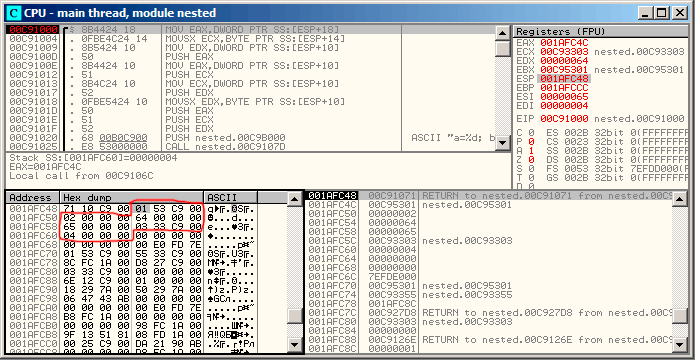
\includegraphics[scale=\FigScale]{patterns/15_structs/5_nested/olly.png}
\caption{\olly: \RU{Перед исполнением \printf}\EN{Before \printf execution}}
\label{fig:nested_olly}
\end{figure}


\section{\RU{Работа с битовыми полями в структуре}\EN{Bit fields in a structure}}

\subsection{\RU{Пример CPUID}\EN{CPUID example}}

\RU{Язык \CCpp позволяет указывать, сколько именно бит отвести для каждого поля структуры. 
Это удобно если нужно экономить место в памяти. К примеру, для переменной типа \Tbool достаточно одного бита.
Но, это не очень удобно, если нужна скорость.}
\EN{\CCpp language allow to define exact number of bits for each structure fields.
It is very useful if one needs to save memory space. 
For example, one bit is enough for variable of \Tbool type.
But of course, it is not rational if speed is important.}

\newcommand{\FNCPUID}{\footnote{\url{http://en.wikipedia.org/wiki/CPUID}}}

\index{x86!\Instructions!CPUID}
\label{cpuid}
\RU{Рассмотрим пример с инструкцией \CPUID\FNCPUID. 
Эта инструкция возвращает информацию о том, какой процессор имеется в наличии и какие возможности он имеет.}
\EN{Let's consider \CPUID\FNCPUID instruction example.
This instruction returning information about current CPU and its features.}

\RU{Если перед исполнением инструкции в \EAX будет 1, 
то \CPUID вернет упакованную в \EAX такую информацию о процессоре:}
\EN{If the \EAX is set to 1 before instruction execution, 
\CPUID will return this information packed into the \EAX register:}

\begin{center}
\begin{tabular}{ | l | l | }
\hline
3:0 (4 \bitsENRU)& Stepping \\
7:4 (4 \bitsENRU) & Model \\
11:8 (4 \bitsENRU) & Family \\
13:12 (2 \bitsENRU) & Processor Type \\
19:16 (4 \bitsENRU) & Extended Model \\
27:20 (8 \bitsENRU) & Extended Family \\
\hline
\end{tabular}
\end{center}

\newcommand{\FNGCCAS}{\footnote{\href{http://www.ibiblio.org/gferg/ldp/GCC-Inline-Assembly-HOWTO.html}
{\RU{Подробнее о встроенном ассемблере GCC}\EN{More about internal GCC assembler}}}}

\RU{MSVC 2010 имеет макрос для \CPUID, а GCC 4.4.1 ~--- нет. 
Поэтому для GCC сделаем эту функцию сами, используя его встроенный ассемблер\FNGCCAS.}
\EN{MSVC 2010 has \CPUID macro, but GCC 4.4.1~---has not.
So let's make this function by yourself for GCC with the help of its built-in assembler\FNGCCAS.}

\lstinputlisting{patterns/15_structs/6_bitfields/cpuid/CPUID.c}

\RU{После того как \CPUID заполнит \EAX/\EBX/\ECX/\EDX, у нас они отразятся в массиве \TT{b[]}. 
Затем, мы имеем указатель на структуру \TT{CPUID\_1\_EAX}, и мы указываем его на значение 
\EAX из массива \TT{b[]}.}
\EN{After \CPUID will fill \EAX/\EBX/\ECX/\EDX, these registers will be reflected in the \TT{b[]} array.
Then, we have a pointer to the \TT{CPUID\_1\_EAX} structure and we point it to the value in the \EAX from \TT{b[]} array.}

\RU{Иными словами, мы трактуем 32-битный \Tint как структуру.}
\EN{In other words, we treat 32-bit \Tint value as a structure.}
\RU{Затем мы читаем из структуры.}\EN{Then we read from the stucture.}

\subsubsection{MSVC}

\RU{Компилируем в MSVC 2008 с опцией \Ox}\EN{Let's compile it in MSVC 2008 with \Ox option}:

\lstinputlisting[caption=\Optimizing MSVC 2008]{patterns/15_structs/6_bitfields/cpuid/CPUID_msvc_Ox.asm}

\index{x86!\Instructions!SHR}
\RU{Инструкция \TT{SHR} сдвигает значение из \EAX на то количество бит, 
которое нужно \IT{пропустить}, то есть, мы игнорируем некоторые биты \IT{справа}.}
\EN{\TT{SHR} instruction shifting value in the \EAX register by number of bits must be
\IT{skipped}, e.g., we ignore some bits \IT{at right}.}

\index{x86!\Instructions!AND}
\RU{А инструкция \ANDIns очищает биты \IT{слева} которые нам не нужны, или же, говоря иначе, 
она оставляет по маске только те биты в \EAX, которые нам сейчас нужны.}
\EN{\ANDIns instruction clears bits not needed \IT{at left}, or, in other words, 
leaves only those bits in the \EAX register we need now.}

\ifdefined\IncludeOlly
\subsubsection{MSVC + \olly}
\index{\olly}

\RU{Загрузим пример в}\EN{Let's load our example into} \olly 
\RU{и увидим, какие значения были установлены в EAX/EBX/ECX/EDX после
исполнения}\EN{and see, which values was set in EAX/EBX/ECX/EDX after execution of} CPUID: 
\figref{fig:cpuid_olly_1}.

\RU{В EAX установлено}\EN{EAX has} \TT{0x000206A7} 
(\RU{мой}\EN{my} \ac{CPU} \EN{is}\RU{---} Intel Xeon E3-1220).\\
\RU{В двоичном виде это}\EN{This is} $0000 0000 0000 0010 0000 0110 1010 0111$\EN{ in binary form}.

\RU{Вот как распределяются биты по полям в моем случае}\EN{Here is how bits are distributed by fields}:

\begin{center}
\begin{tabular}{ | l | l | l | }
\hline
\headercolor{} \RU{поле}\EN{field} &
\headercolor{} \RU{в двоичном виде}\EN{in binary form} &
\headercolor{} \RU{в десятичном виде}\EN{in decimal form} \\
\hline
reserved2		& 0000 & 0 \\
\hline
extended\_family\_id	& 00000000 & 0 \\
\hline
extended\_model\_id	& 0010 & 2 \\
\hline
reserved1		& 00 & 0 \\
\hline
processor\_id		& 00 & 0 \\
\hline
family\_id		& 0110 & 6 \\
\hline
model			& 1010 & 10 \\
\hline
stepping		& 0111 & 7 \\
\hline
\end{tabular}
\end{center}

\begin{figure}[H]
\centering
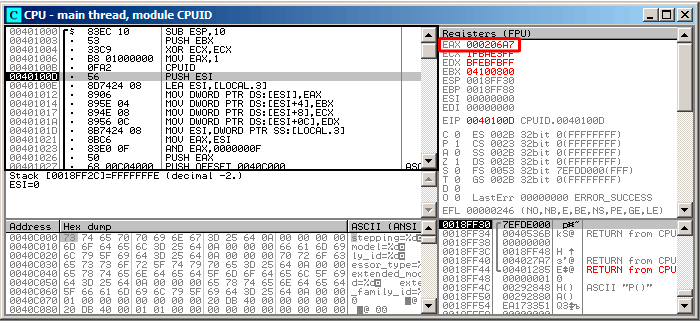
\includegraphics[scale=\FigScale]{patterns/15_structs/6_bitfields/cpuid/olly.png}
\caption{\olly: \RU{После исполнения CPUID}\EN{After CPUID execution}}
\label{fig:cpuid_olly_1}
\end{figure}

\begin{figure}[H]
\centering
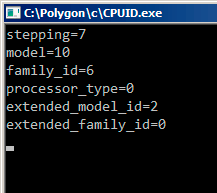
\includegraphics[scale=0.66]{patterns/15_structs/6_bitfields/cpuid/result.png}
\caption{\olly: \RU{Результат работы}\EN{Result}}
\label{fig:cpuid_olly_2}
\end{figure}
\fi

\subsubsection{GCC}

\RU{Попробуем GCC 4.4.1 с опцией \Othree.}\EN{Let's try GCC 4.4.1 with \Othree option.}

\lstinputlisting[caption=\Optimizing GCC 4.4.1]{patterns/15_structs/6_bitfields/cpuid/CPUID_gcc_O3.asm}

\RU{Практически, то же самое. Единственное что стоит отметить это то, что GCC решил зачем-то объединить 
вычисление \TT{extended\_model\_id} и \TT{extended\_family\_id} в один блок, 
вместо того чтобы вычислять их перед соответствующим вызовом \printf.}
\EN{Almost the same.
The only thing worth noting is the GCC somehow united calculation of
\TT{extended\_model\_id} and \TT{extended\_family\_id} into one block,
instead of calculating them separately, before corresponding each \printf call.}

\subsection{\WorkingWithFloatAsWithStructSubSubSectionName}
\label{sec:floatasstruct}

\RU{Как уже ранее указывалось в секции о FPU~(\myref{sec:FPU}), 
и \Tfloat и \Tdouble содержат в себе \IT{знак}, \IT{мантиссу} и \IT{экспоненту}. 
Однако, можем ли мы работать с этими полями напрямую? Попробуем с \Tfloat.}
\EN{As we already noted in the section about FPU~(\myref{sec:FPU}), 
both \Tfloat and \Tdouble types consist of a \IT{sign}, 
a \IT{significand} (or \IT{fraction}) and an \IT{exponent}.
But will we be able to work with these fields directly? Let's try this with \Tfloat.}

\bigskip
% a hack used here! http://tex.stackexchange.com/questions/73524/bytefield-package
\begin{center}
\begin{bytefield}{32}
	\bitheader[endianness=big]{0,22,23,30,31} \\
	\bitbox{1}{S} & 
	\bitbox{8}{%
		\RU{экспонента}%
		\EN{exponent}%
		\ES{exponente}%
		\PTBRph{}%
		\DEph{}\PLph{}%
		\ITAph{}%
		\FR{exposant}
	} & 
	\bitbox{23}{%
		\RU{мантисса}%
		\EN{mantissa or fraction}%
		\ES{mantisa o fracci\'on}%
		\PTBRph{}%
		\DEph{}\PLph{}%
		\ITAph{}%
		\FR{mantisse ou fraction}
	}
\end{bytefield}
\end{center}

\begin{center}
( S\EMDASH{}%
	\RU{знак}%
	\EN{sign}%
	\ES{signo}%
	\PTBRph{}%
	\DEph{}\PLph{}%
	\ITAph{}%
	\FR{signe}
)
\end{center}


\lstinputlisting{patterns/15_structs/6_bitfields/float/float.c.\LANG}

\RU{Структура \TT{float\_as\_struct} занимает в памяти столько же места сколько и \Tfloat, 
то есть 4 байта или 32 бита.}
\EN{The \TT{float\_as\_struct} structure occupies the same amount of  memory as \Tfloat, i.e., 4 bytes or 32 bits.}

\RU{Далее мы выставляем во входящем значении отрицательный знак, 
а также прибавляя двойку к экспоненте, мы тем 
самым умножаем всё значение на \TT{$2^2$}, то есть на 4.}
\EN{Now we are setting the negative sign in the input value and also, by adding 2 to the exponent, 
we thereby multiply the whole number by \TT{$2^2$}, i.e., by 4.}

\RU{Компилируем в MSVC 2008 без включенной оптимизации:}
\EN{Let's compile in MSVC 2008 without optimization turned on:}

\lstinputlisting[caption=\NonOptimizing MSVC 2008]{patterns/15_structs/6_bitfields/float/float_msvc.asm.\LANG}

\RU{Слегка избыточно. В версии скомпилированной с флагом \Ox нет вызовов \TT{memcpy()}, 
там работа происходит сразу с переменной \TT{f}. Но по неоптимизированной версии будет проще понять.}
\EN{A bit redundant.
If it was compiled with \Ox flag there would be no \TT{memcpy()} call,
the \TT{f} variable is used directly.
But it is easier to understand by looking at the unoptimized version.}

\RU{А что сделает GCC 4.4.1 с опцией \Othree?}\EN{What would GCC 4.4.1 with \Othree do?}

\lstinputlisting[caption=\Optimizing GCC 4.4.1]{patterns/15_structs/6_bitfields/float/float_gcc_O3.asm.\LANG}

\RU{Да, функция \ttf в целом понятна. Однако, что интересно, еще при компиляции, 
не взирая на мешанину с полями структуры, GCC умудрился вычислить результат функции \TT{f(1.234)} еще
во время компиляции и сразу подставить его в аргумент для \printf{}!}
\EN{The \ttf function is almost understandable. However, what is interesting is that GCC was able to calculate
the result of \TT{f(1.234)} during compilation despite all this hodge-podge with the structure fields
and prepared this argument to \printf{} as precalculated at compile time!}


\subsection{\Exercises}

\begin{itemize}
	\item \url{http://challenges.re/71}
	\item \url{http://challenges.re/72}
\end{itemize}



